\documentclass[11pt]{article}
\usepackage[utf8]{inputenc}
\usepackage[T1]{fontenc}
\usepackage[margin=0.78in]{geometry}
\usepackage{graphicx}
\usepackage{booktabs}
\usepackage{tabularx}
\usepackage{array}
\usepackage{float}
\usepackage{xcolor}
\AtBeginDocument{\color{black}}
\usepackage{hyperref}
\hypersetup{hidelinks}
\setlength{\parskip}{5pt}
\setlength{\parindent}{0pt}
\pagestyle{plain}

\begin{document}

{\Large\bfseries Tornado Risk and Home-Purchasing Patterns in Central Iowa}\par
{\large Ames housing sales and tornado activity, 2005-2010}\par
\vspace{3pt}
\vspace{10pt}

\section*{Executive summary}
This analysis asks whether home-purchasing patterns in Ames, Iowa, differ in months when tornadoes were recorded in Story County and six surrounding counties, and whether the relationship varies for homes with basements. The housing data contain 2,884 sales from January 2006 through July 2010. In those 55 sale months, 9 months had at least one recorded tornado in the seven-county region and 46 had none. The tornado file contains 37 events in the selected years 2005-2010; 21 occurred during the housing period's 9 active months.

The models did not detect a statistically significant association between tornado-active months and the chance that a purchased home had a basement (odds ratio 0.734, 95\% CI 0.411-1.309, cluster-robust $p=0.295$). A factorial sale-price model also found no detectable tornado-month effect ($p=0.5366$) or interaction between tornado activity and basement status ($p=0.7250$), after controlling for sale year and calendar month.

There is a clear overall price difference between the basement groups: the median sale price was \$162,000 for homes with basements and \$100,000 for homes without one. The estimated median gap was \$62,000 (95\% bootstrap CI \$52,000-\$67,841). This is an unadjusted association, not an estimate of what buyers paid specifically for basement safety. Only 77 of 2,884 homes (2.7\%) lacked a basement, so estimates for that group are comparatively imprecise.

\textbf{Main takeaway:} In this sample, we found no statistically detectable evidence that recorded tornado activity changed the likelihood of buying a home with a basement or changed the basement-related sale-price pattern. This does not establish that tornado risk has no effect. The study has only 9 active sale months, uses a broad regional tornado measure for Ames sales, and does not observe buyers' stated motivations.

\section*{Data and scope}
\begin{itemize}
  \item \textbf{Housing:} 2,884 Ames home sales, January 2006-July 2010. The dataset has 82 fields, including sale price, sale month, and total basement area.
  \item \textbf{Tornadoes:} event records for Story, Hamilton, Hardin, Marshall, Jasper, Polk, and Boone counties. The working file contains 435 events across all years; 37 tornadoes were recorded in 2005-2010 across the seven counties.
  \item \textbf{Tornado month:} a calendar month with one or more tornado records in any of the seven counties. Multiple tornadoes in one month count as one active month for the binary models.
  \item \textbf{Basement:} a home is coded as having a basement when \texttt{Total Bsmt SF} is greater than zero.
\end{itemize}
The housing data begin in 2006, so 2005 appears in tornado visualizations but has no corresponding housing observations. The model sample therefore contains 55 housing months: 9 tornado-active months and 46 non-tornado months.

\section*{Housing and tornado patterns over time}
Monthly sales volume shows a recurring rise during warmer months and a decline in winter. Average sale price varies substantially month to month. The tornado series is sparse: among the 37 events recorded from 2005-2010, June and November each contain 13 events. The shared calendar axes make timing visible, but the measures use separate scales and visual co-movement alone does not show that tornado activity affects purchase choices.

\begin{figure}[H]
\centering
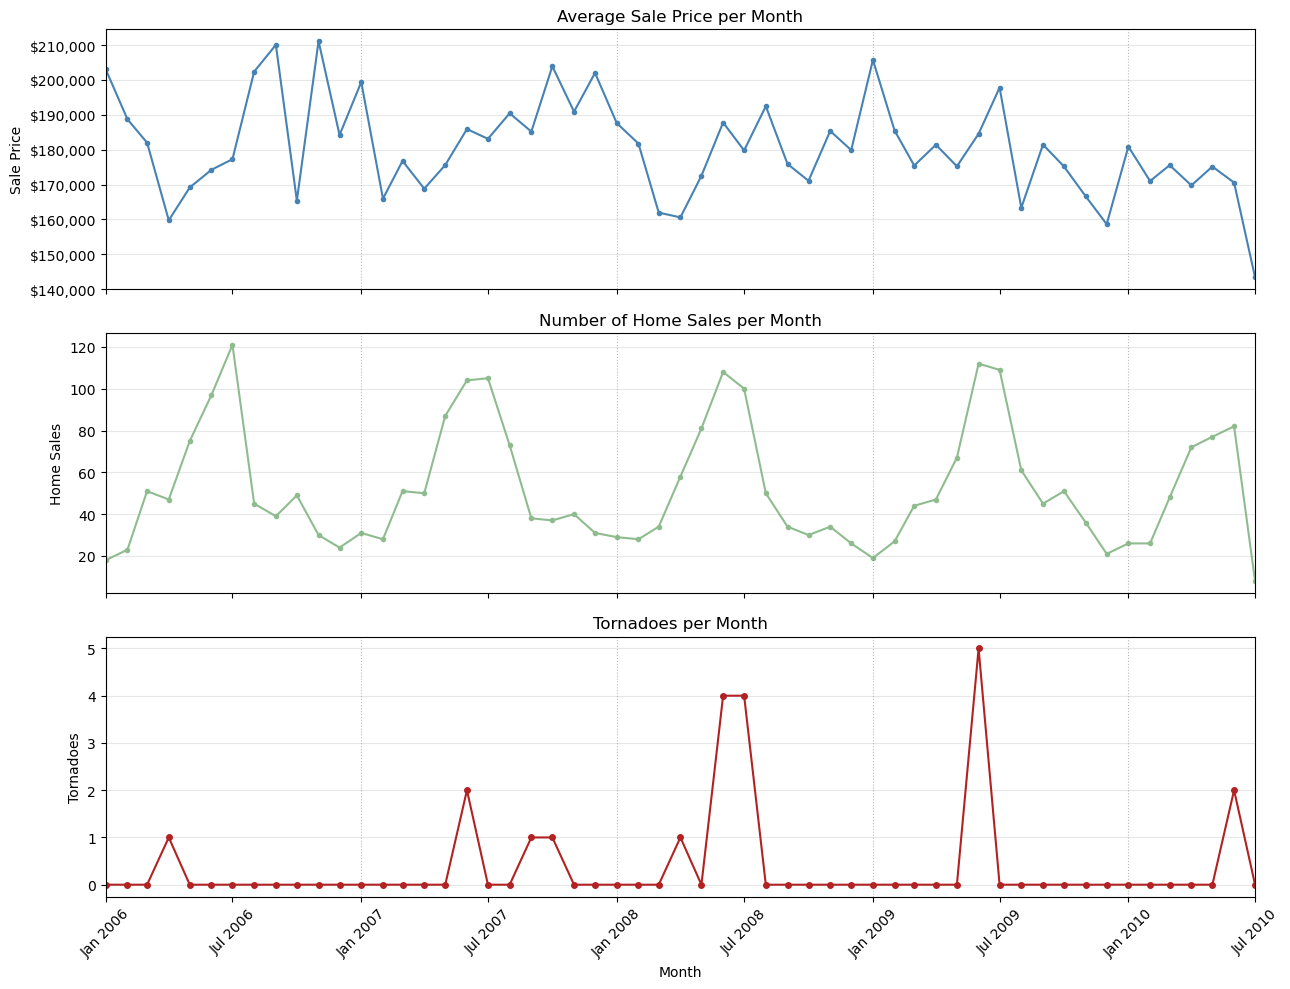
\includegraphics[width=0.96\textwidth]{../analysis/ames_tornado_report_assets/housing_tornado_comparison.png}
\caption{Monthly housing price, sales volume, and tornado counts on a shared January 2006-July 2010 timeline. Each panel has its own vertical scale.}
\end{figure}

\section*{Basement purchases around tornado months}
For each of the 9 active tornado months that overlap housing sales, purchases in the immediately preceding month, the tornado month, and the following month were summarized. The table is descriptive. Windows around different tornado months may overlap, and the before/during/after rows should not be treated as independent experimental groups.

\begin{table}[H]
\centering
\footnotesize
\setlength{\tabcolsep}{3pt}
\begin{tabularx}{\textwidth}{lrrrr>{\raggedleft\arraybackslash}X>{\raggedleft\arraybackslash}X}
\toprule
Window & Purchases & Basement & No basement & No-basement share & Median w/ basement & Median w/o basement \\
\midrule
Month before & 616 & 605 & 11 & 1.8\% & \$161,000 & \$89,500 \\
Tornado month & 686 & 660 & 26 & 3.8\% & \$165,200 & \$116,290 \\
Month after & 605 & 590 & 15 & 2.5\% & \$164,700 & \$98,300 \\
\bottomrule
\end{tabularx}
\caption{Home sales around unique tornado-active calendar months. Median basement price differences were \$71,500 before, \$48,910 during, and \$66,400 after.}
\end{table}

The observed no-basement share rises from 1.8\% before to 3.8\% during the active month, then is 2.5\% after. The groups without basements are small (11, 26, and 15 homes), so these percentages and median prices are sensitive to a small number of sales. The modeled basement-by-tornado interaction is not statistically significant, so this descriptive dip does not establish a change in buyers' preferences.

\begin{figure}[H]
\centering
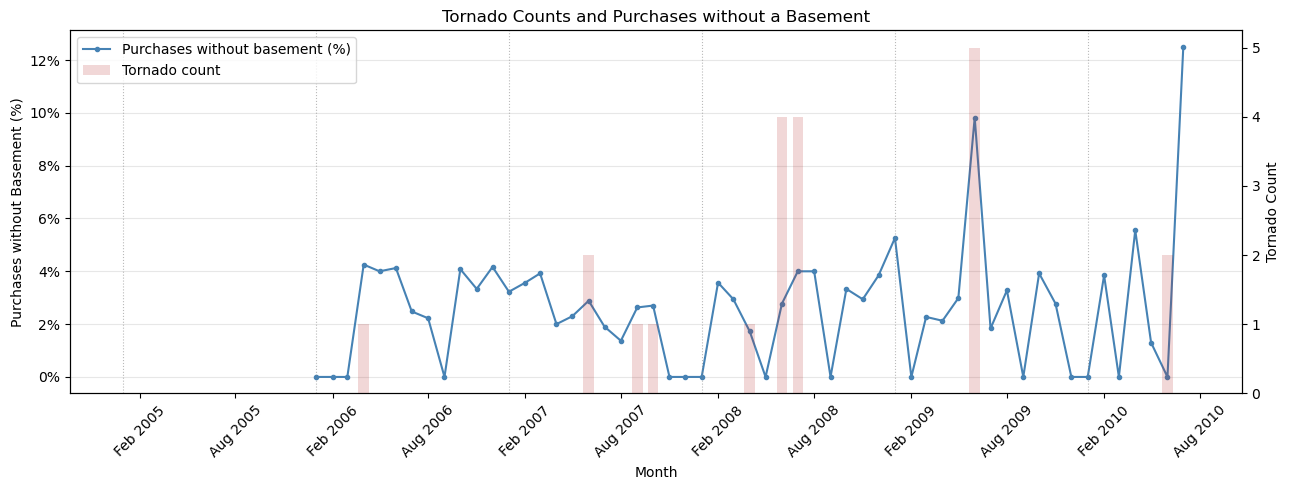
\includegraphics[width=0.96\textwidth]{../analysis/ames_tornado_report_assets/tornado_no_basement_timeline.png}
\caption{Monthly tornado counts and the percentage of Ames purchases without a basement. The housing series is blank before housing data begin.}
\end{figure}

\begin{figure}[H]
\centering
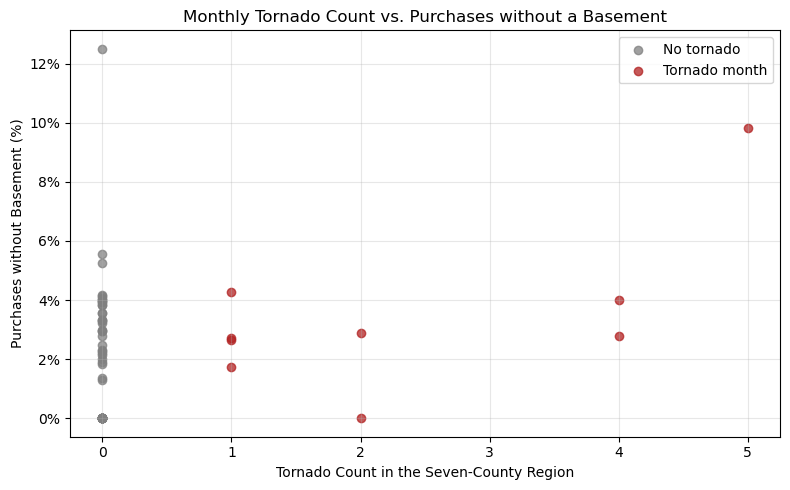
\includegraphics[width=0.72\textwidth]{../analysis/ames_tornado_report_assets/tornado_no_basement_scatter.png}
\caption{Monthly tornado count versus the share of purchases without a basement. The July 2010 share is 1 of 8 purchases, illustrating how small monthly samples can produce large percentage swings.}
\end{figure}

Across all observed sale months, 26 of 686 purchases in tornado months (3.79\%) lacked a basement, compared with 51 of 2,198 purchases in non-tornado months (2.32\%). This difference is descriptive; the regression below accounts for calendar month and year and gives a non-significant result.

\section*{Statistical tests}
\subsection*{Logistic regression: basement purchase}
The binary outcome is 1 for a home with a basement and 0 for a home without one. Tornado-month status is the main predictor. The model controls for sale year and calendar month; standard errors are clustered by sale month because every sale in a month shares the same tornado status.

\begin{table}[H]
\centering
\small
\begin{tabularx}{\textwidth}{lrrrX}
\toprule
Outcome & Odds ratio & 95\% CI & $p$ & Result \\
\midrule
Basement purchase (tornado vs. other months) & 0.734 & 0.411-1.309 & 0.2950 & Not statistically significant \\
\bottomrule
\end{tabularx}
\end{table}
The point estimate corresponds to lower odds of a basement purchase in a tornado month, but the confidence interval includes 1 and the test is not statistically significant. With only 9 tornado-active months, the estimate is uncertain.

\subsection*{Factorial sale-price model}
The sale-price model includes basement status, tornado-month status, their interaction, sale-year controls, and calendar-month controls. Cluster-robust Wald term tests are used for the three terms of interest. The basement term is statistically significant, but the tornado-month and interaction terms are not.

\begin{table}[H]
\centering
\small
\begin{tabularx}{\textwidth}{lrrX}
\toprule
Model term & Wald stat. & $p$-value & Reading \\
\midrule
Basement status & 209.486 & $<0.0001$ & Sale prices differ by basement status in this model \\
Tornado-month status & 0.382 & 0.5366 & No detected sale-price difference by tornado status \\
Basement $\times$ tornado month & 0.124 & 0.7250 & No detected change in the basement price pattern \\
\bottomrule
\end{tabularx}
\end{table}

The statistically significant basement term does not show that buyers paid for safety: homes with basements can differ in size, quality, age, location, and other sale-relevant features. Those property characteristics were not included in this analysis. The tornado and interaction terms are the relevant tests for whether the observed tornado-month status is associated with sale prices or with a changed basement price pattern; neither is significant here.

\section*{Conclusion and limits}
The results support a restrained conclusion: within the observed 2006-2010 Ames sales, tornado-active months were not associated with statistically detectable changes in basement-purchase odds or in sale-price patterns after accounting for calendar month and year. The data show seasonal structure in both home sales and tornado records, but shared seasonality is not evidence that tornado threats drive purchase decisions.

The conclusion is limited by the short observation period, only 9 active sale months, the small no-basement group, and the use of tornado counts from seven counties as a common monthly exposure for Ames housing sales. The data do not measure buyer beliefs or safety motivations. Non-significant tests mean that this analysis did not detect an association; they do not prove that no effect exists.

\textbf{Data files:} \texttt{AmesHousing-working.csv} and \texttt{Iowa-central-counties-tornadoes-working.csv}. Basement price differences and event-window summaries are unadjusted unless the model description states otherwise.

\end{document}


